\documentclass[tikz,border=5pt]{standalone}
\usepackage{amsmath}
\usetikzlibrary{arrows.meta,matrix}

\begin{document}
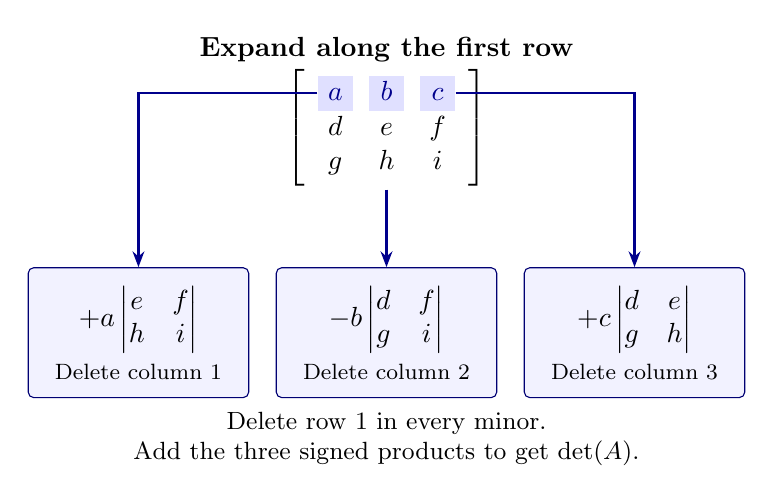
\begin{tikzpicture}[
  term/.style={draw=blue!45!black, fill=blue!5, rounded corners=2pt,
    minimum width=2.8cm, minimum height=1.65cm, align=center},
  guide/.style={blue!55!black, thick, -{Stealth[length=2mm]}}
]
  \node[font=\bfseries] at (0,2.9) {Expand along the first row};
  \matrix (A) [matrix of math nodes, left delimiter={[}, right delimiter={]},
    column sep=0.21cm,
    nodes={minimum size=0.44cm, inner sep=0pt, text height=1.7ex, text depth=0.5ex},
    row 1/.style={nodes={fill=blue!12, text=blue!55!black}}] at (0,1.9) {
    a & b & c \\
    d & e & f \\
    g & h & i \\
  };
  \node[term] (first) at (-3.15,-0.7)
    {\(\displaystyle +a\begin{vmatrix}e&f\\h&i\end{vmatrix}\)\\[3pt]
     \footnotesize Delete column 1};
  \node[term] (second) at (0,-0.7)
    {\(\displaystyle -b\begin{vmatrix}d&f\\g&i\end{vmatrix}\)\\[3pt]
     \footnotesize Delete column 2};
  \node[term] (third) at (3.15,-0.7)
    {\(\displaystyle +c\begin{vmatrix}d&e\\g&h\end{vmatrix}\)\\[3pt]
     \footnotesize Delete column 3};

  \draw[guide] (A-1-1.west) -- ++(-0.75,0) -| (first.north);
  \draw[guide] (A.south) -- (second.north);
  \draw[guide] (A-1-3.east) -- ++(0.75,0) -| (third.north);
  \node[font=\small, align=center] at (0,-2.05)
    {Delete row 1 in every minor.\\Add the three signed products to get \(\det(A)\).};
\end{tikzpicture}
\end{document}
